\section*{Άσκηση 2}
\label{ex2}
\addcontentsline{toc}{section}{\nameref{ex2}}

\subsection*{Ερώτημα 1}
\label{ex2q1}
\addcontentsline{toc}{subsection}{\nameref{ex2q1}}

Σύμφωνα με τα δεδομένα της εκφώνησης η Discrete Time Markov Chain σχεδιάζεται ως εξής:\\\\

\begin{figure}[!h]
	\begin{center}
		\begin{tikzpicture}
			\node [circle,draw, minimum size=0.5cm] at (2,  0) (W) {W};
			\node [circle,draw, minimum size=0.78cm] at (5, -1.5) (S) {S};
			\node [circle,draw, minimum size=0.5cm] at (5,  1.5) (B) {B};

			\draw [-Triangle, thick] ($(W) + (0.2, 0.37)$) -- ($(B) + (-0.33, 0.15)$) node [pos=0.3, above] {$\frac{1}{6}$};
			\draw [-Triangle, thick] ($(B) + (-0.3, -0.22)$) -- ($(W) + (0.41, 0.1)$) node [pos=0.3, below] {1};
			
			\draw [-Triangle, thick] ($(W) + (0.37, -0.18)$) -- ($(S) + (-0.32, 0.2)$) node [pos=0.3, above] {$\frac{1}{4}$};
			\draw [-Triangle, thick] ($(S) + (-0.37, -0.13)$) -- ($(W) + (0.12, -0.4)$) node [pos=0.3, below] {$\frac{3}{4}$};

			\path (S) edge [loop right, thick, -Triangle, in=0, out=60, looseness=6] node [above, sloped, pos=0.25] (TextNode1) {$\frac{1}{4}$} (S);
			\path (W) edge [loop right, thick, -Triangle, in=165, out=110, looseness=6] node [above, sloped, pos=0.32] (TextNode1) {$\frac{7}{12}$} (W);
		\end{tikzpicture}
	\end{center}
	\caption{Discrete Markov Chain}
	\label{DTMC}
\end{figure}

\subsection*{Ερώτημα 2}
\label{ex2q2}
\addcontentsline{toc}{subsection}{\nameref{ex2q2}}

Για να είναι εργοτική η DTMC του figure 3 είναι απαραίτητο να ισχύουν οι εξής προϋποθέσεις:
\begin{enumerate}
	\item Recurrent (Ελληνικά)
	\item Απεριοδική
	\item All nodes communicating to each other
\end{enumerate}

\noindent\\
\textbf{Recurrent}\\
H DTMC είναι Recurrent εφόσον δεν υπάρχει κάποιο state το οποίο είναι transient, δηλαδή δεν υπάρχει κάποιο state από το οποίο αν γίνει μετάβαση από αυτό, δεν είναι εφικτή η επιστροφή σε αυτό.\\

\noindent\\
\textbf{Απεριοδικότητα}\\
Η DTMC είναι Απεριοδική εφόσον δεν υπάρχει κάποιο state το οποίο είναι περιοδικό, δηλαδή δεν υπάρχει κάποιο state από το οποίο όλα τα πιθανά μονοπάτια που ξεκινούν και καταλήγουν σε αυτό να είναι πολλαπλάσια του ίδιου αριθμού Κ (Κ$>$1). Αυτό συμβαίνει καθώς υπάρχουν self loops σε 2 από τα 3 states με αποτέλεσμα η μετάβαση να μπορεί να μεγαλώσει αρκετά αξιοποιώντας τα.\\

\noindent
π.χ. για το state Β, η μετάβαση $B \xrightarrow[]{} W \xrightarrow[]{} B$ έχει ελάχιστο μήκος διαδρομής, ίσο με 2, όμως αντίστοιχα μπορεί\\ \vspace{1cm} \qquad να εκτελεστεί και η διαδρομή $B \xrightarrow[]{} W \xrightarrow[]{} W \xrightarrow[]{} B$ η οποία έχει μήκος ίσο με 3.

\noindent
\textbf{All nodes connect with each other}\\
Από το figure (\ref{DTMC}) είναι εμφανές πως όλοι οι κόμβοι επικοινωνούν μεταξύ τους, δηλαδή από κάθε ένα κόμβο, μπορεί να γίνει μετάβαση σε έναν άλλο.


\noindent\\\\\\
Άρα, πληρούνται όλες οι προϋποθέσεις και ως αποτέλεσμα η DTMC είναι εργοτική

\clearpage
\subsection*{Ερώτημα 3}
\label{ex2q3}
\addcontentsline{toc}{subsection}{\nameref{ex2q3}}

Για να είναι χρονικά-αναστρέψιμη η DTMC πρέπει να ισχύει το local balance. Εφαρμόζοντας local balance σε κάθε ζευγάρι κόμβων προκύπτουν οι εξής σχέσεις:
\begin{align}
	P_W \cdot \frac{1}{6} = P_B \cdot 1 &\xRightarrow{} P_B = P_W \cdot \frac{1}{6} \label{pbw}\\
	P_W \cdot \frac{1}{4} = P_S \cdot \frac{3}{4} &\xRightarrow{} P_S = P_W \cdot \frac{1}{3} \label{psw}
\end{align}

\noindent\\
Ακόμα, πρέπει να ισχύει η εξής σχέση:
\begin{align*}
	P_W + P_B + P_S = 1
\end{align*}

οπότε αντικαθιστώντας τις σχέσεις (\ref{pbw}), (\ref{psw}) προκύπτουν τα εξής αποτελέσματα:
\begin{align}
	P_W + P_B + P_S = 1 &\xRightarrow{} P_W + P_W \cdot \frac{1}{6} + P_W \cdot \frac{1}{3} = 1 \notag \xRightarrow{}\\
						&\xRightarrow{} P_W \left( \frac{6}{6} + \frac{1}{6} +  \frac{2}{6} \right) = 1 \notag \xRightarrow{}\\
						&\xRightarrow{} P_W \left( \frac{3}{2} \right) = 1 \notag \xRightarrow{}\\
						&\xRightarrow{} P_W = \frac{2}{3} \label{PW}
\end{align}

και από τις σχέσεις (\ref{pbw}), (\ref{psw}) οι τιμές των $P_S$ και $P_B$ προκύπτουν ως εξής:
\begin{align}
	\xRightarrow[(\ref{pbw})]{(\ref{PW})} P_B = P_W \cdot \frac{1}{6} = \frac{2}{3} \cdot \frac{1}{6} \xRightarrow{} P_B = \frac{1}{9}\\
	\xRightarrow[(\ref{psw})]{(\ref{PW})} P_S = P_W \cdot \frac{1}{3} = \frac{2}{3} \cdot \frac{1}{3} \xRightarrow{} P_S = \frac{2}{9}
\end{align}


\noindent\\
Εφόσον οι τιμές των $P_W$, $P_B$, $P_S$ είναι μικρότερες του 1 και το άθροισμά τους είναι ίσο με 1, τότε ισχύει το local balance και κατ' εξοχήν η DTMC είναι χρονικά-αναστρέψιμη.

\subsection*{Ερώτημα 4}
\label{ex2q4}
\addcontentsline{toc}{subsection}{\nameref{ex2q4}}

Ο χρόνος για τον οποίο θα λειτουργεί το data center είναι ο χρόνος που θα βρίσκεται στο state W, το οποίο σύμφωνα με το προηγούμενο ερώτημα, η πιθανότητα να βρίσκεται στο $P_W$ είναι ίσο με $\frac{2}{3}$, δηλαδή το data center θα είναι ενεργό το 66,6\% του χρόνου.


\subsection*{Ερώτημα 5}
\label{ex2q5}
\addcontentsline{toc}{subsection}{\nameref{ex2q5}}



\begin{figure}
	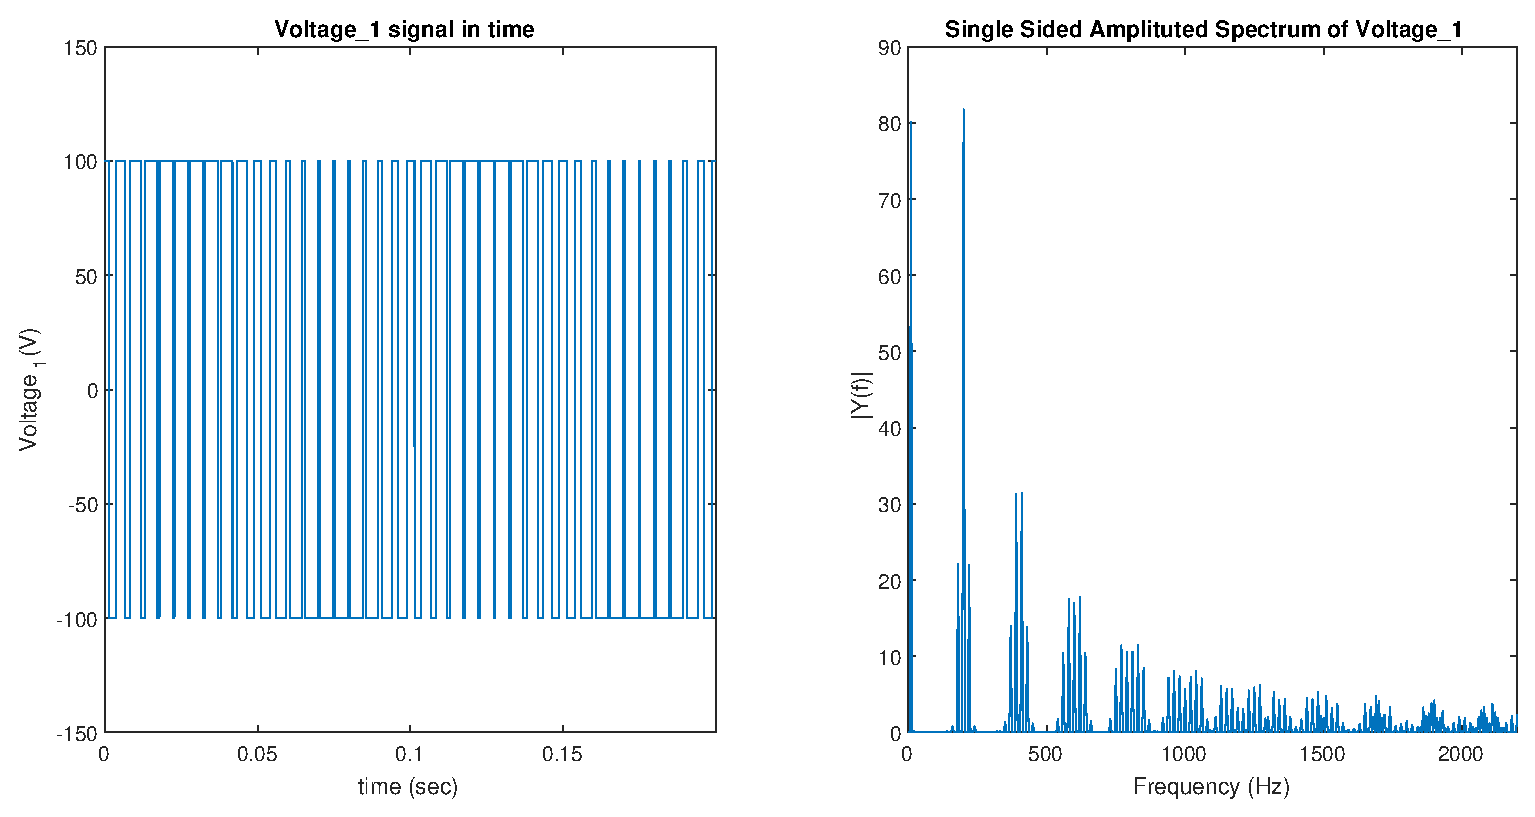
\includegraphics[width=\textwidth]{voltage1_Q3.eps} 
\end{figure} 

τι κάνεις γαμώ την παναγία σου 